% Options for packages loaded elsewhere
\PassOptionsToPackage{unicode}{hyperref}
\PassOptionsToPackage{hyphens}{url}
\documentclass[
  ignorenonframetext,
]{beamer}
\newif\ifbibliography
\usepackage{pgfpages}
\setbeamertemplate{caption}[numbered]
\setbeamertemplate{caption label separator}{: }
\setbeamercolor{caption name}{fg=normal text.fg}
\beamertemplatenavigationsymbolsempty
% remove section numbering
\setbeamertemplate{part page}{
  \centering
  \begin{beamercolorbox}[sep=16pt,center]{part title}
    \usebeamerfont{part title}\insertpart\par
  \end{beamercolorbox}
}
\setbeamertemplate{section page}{
  \centering
  \begin{beamercolorbox}[sep=12pt,center]{section title}
    \usebeamerfont{section title}\insertsection\par
  \end{beamercolorbox}
}
\setbeamertemplate{subsection page}{
  \centering
  \begin{beamercolorbox}[sep=8pt,center]{subsection title}
    \usebeamerfont{subsection title}\insertsubsection\par
  \end{beamercolorbox}
}
% Prevent slide breaks in the middle of a paragraph
\widowpenalties 1 10000
\raggedbottom
\AtBeginPart{
  \frame{\partpage}
}
\AtBeginSection{
  \ifbibliography
  \else
    \frame{\sectionpage}
  \fi
}
\AtBeginSubsection{
  \frame{\subsectionpage}
}
\usepackage{iftex}
\ifPDFTeX
  \usepackage[T1]{fontenc}
  \usepackage[utf8]{inputenc}
  \usepackage{textcomp} % provide euro and other symbols
\else % if luatex or xetex
  \usepackage{unicode-math} % this also loads fontspec
  \defaultfontfeatures{Scale=MatchLowercase}
  \defaultfontfeatures[\rmfamily]{Ligatures=TeX,Scale=1}
\fi
\usepackage{lmodern}
\usetheme[]{Madrid}
\usefonttheme[]{professionalfonts}
\ifPDFTeX\else
  % xetex/luatex font selection
\fi
% Use upquote if available, for straight quotes in verbatim environments
\IfFileExists{upquote.sty}{\usepackage{upquote}}{}
\IfFileExists{microtype.sty}{% use microtype if available
  \usepackage[]{microtype}
  \UseMicrotypeSet[protrusion]{basicmath} % disable protrusion for tt fonts
}{}
\makeatletter
\@ifundefined{KOMAClassName}{% if non-KOMA class
  \IfFileExists{parskip.sty}{%
    \usepackage{parskip}
  }{% else
    \setlength{\parindent}{0pt}
    \setlength{\parskip}{6pt plus 2pt minus 1pt}}
}{% if KOMA class
  \KOMAoptions{parskip=half}}
\makeatother
% definitions for citeproc citations
\NewDocumentCommand\citeproctext{}{}
\NewDocumentCommand\citeproc{mm}{%
  \begingroup\def\citeproctext{#2}\cite{#1}\endgroup}
\makeatletter
 % allow citations to break across lines
 \let\@cite@ofmt\@firstofone
 % avoid brackets around text for \cite:
 \def\@biblabel#1{}
 \def\@cite#1#2{{#1\if@tempswa , #2\fi}}
\makeatother
\newlength{\cslhangindent}
\setlength{\cslhangindent}{1.5em}
\newlength{\csllabelwidth}
\setlength{\csllabelwidth}{3em}
\newenvironment{CSLReferences}[2] % #1 hanging-indent, #2 entry-spacing
 {\begin{list}{}{%
  \setlength{\itemindent}{0pt}
  \setlength{\leftmargin}{0pt}
  \setlength{\parsep}{0pt}
  % turn on hanging indent if param 1 is 1
  \ifodd #1
   \setlength{\leftmargin}{\cslhangindent}
   \setlength{\itemindent}{-1\cslhangindent}
  \fi
  % set entry spacing
  \setlength{\itemsep}{#2\baselineskip}}}
 {\end{list}}
\usepackage{calc}
\newcommand{\CSLBlock}[1]{\hfill\break\parbox[t]{\linewidth}{\strut\ignorespaces#1\strut}}
\newcommand{\CSLLeftMargin}[1]{\parbox[t]{\csllabelwidth}{\strut#1\strut}}
\newcommand{\CSLRightInline}[1]{\parbox[t]{\linewidth - \csllabelwidth}{\strut#1\strut}}
\newcommand{\CSLIndent}[1]{\hspace{\cslhangindent}#1}
\setlength{\emergencystretch}{3em} % prevent overfull lines
\providecommand{\tightlist}{%
  \setlength{\itemsep}{0pt}\setlength{\parskip}{0pt}}
\usepackage{xurl}          % better URL/DOI wrapping
\usepackage{microtype}     % nicer spacing
\setbeamertemplate{bibliography item}[text]  % no bullets on refs
\usepackage{bookmark}
\IfFileExists{xurl.sty}{\usepackage{xurl}}{} % add URL line breaks if available
\urlstyle{same}
\hypersetup{
  pdftitle={An adaptive test based on Kendall's tau for independence in high dimensions},
  pdfauthor={Sam Olson},
  hidelinks,
  pdfcreator={LaTeX via pandoc}}

\title{An adaptive test based on Kendall's tau for independence in high
dimensions}
\author{Sam Olson}
\date{}

\begin{document}
\frame{\titlepage}

\begin{frame}{Synopsis of Paper}
\phantomsection\label{synopsis-of-paper}
\begin{itemize}
\tightlist
\item
  Testing the mutual independence for high-dimensional data.
\item
  Known that \(L_2\)-type statistics have lower power under sparse
  alternatives and \(L_\infty\)-type statistics have lower power under
  dense alternatives in high dimensions.
\item
  With this in mind, develop an adaptive test based on Kendall's
  \(\tau\) to compromise both situations of the alternative, which can
  automatically be adapted to the underlying data.
\item
  Establish the asymptotic joint distribution of \(L_2\)-type and
  \(L_\infty\)-type statistics based on Kendall's \(\tau\) under mild
  assumptions and the asymptotic null distribution of the proposed
  statistic.
\item
  Apply simulation to assess how well the test does compared to other
  testing methods, results that indicate the adaptive test performs well
  in either dense or sparse cases.
\end{itemize}
\end{frame}

\begin{frame}{What is Kendall's \(\tau\)}
\phantomsection\label{what-is-kendalls-tau}
\[
\tau = \frac{(\text{Count of concordant pairs}) - (\text{Count of discordant pairs})}{(\text{Number of pairs})}
\]

\begin{itemize}
\tightlist
\item
  Where concordant: Text
\item
  And where discordant: Text
\item
  There are other types of Kendall's \(\tau\), e.g., \(\tau-a\),
  \(\tau-b\), \(\tau-c\)
\end{itemize}
\end{frame}

\begin{frame}{How Does This Fit Into a Broader Narrative?}
\phantomsection\label{how-does-this-fit-into-a-broader-narrative}
\begin{itemize}
\tightlist
\item
  \textbf{1897} --- Fechner introduces the \emph{method of signs} for
  succession-dependence.
\item
  \textbf{1938} --- Kendall develops the \(\tau\) rank correlation
  coefficient.
\item
  \textbf{1958} --- Kruskal broadens Kendall's ideas into a general
  nonparametric testing framework.
\item
  \textbf{1958--1990s} --- Others (e.g., El-Shaarawi, 1992) apply
  rank-based methods to time series.
\item
  \textbf{2024} --- Shi et al.~develop adaptive high-dimensional
  independence tests using Kendall's \(\tau\).
\item
  \textbf{2025} --- Han et al.~extend to a broader class of
  sum-of-powers tests.
\end{itemize}
\end{frame}

\begin{frame}[allowframebreaks]{General Summary}
\phantomsection\label{general-summary}
In \emph{Kollektivmasslehre} (Fechner 1897) created a ``precursor'' to
Kendall's \(\tau\). His method of signs looked for
consecutive-dependence in sequences of observations: Assess concordance
and discordance using only the signs of differences, not their
magnitudes.

Kendall (Kendall 1938) generalized Fechner's idea by considering all
possible pairs of observations, not just consecutive ones. His \(\tau\)
statistic became the canonical rank correlation coefficient, widely
adopted as a nonparametric alternative to Pearson's correlation.

Kruskal (Kruskal 1958) emphasized \(\tau\)'s place within a broader
family of nonparametric statistics for ordinal data, within the
framework of formal hypothesis testing.

Rank-based measures then spread to time series, enabling tests for
persistence/independence in various settings (El-Shaarawi and Niculescu
1992; Hamed 2011).

And now, we apply these methods (use Kendall's \(\tau\)) for the
purposes of robust, distribution-free procedures, assessing both how and
under what circumstances these tests of independence may be applied
(e.g., whether the type of data or problem would lend itself to such an
application) (Shi et al. 2024; Han, Ma, and Xie 2025).
\end{frame}

\begin{frame}{How Is This Non-Parametric?}
\phantomsection\label{how-is-this-non-parametric}
\begin{itemize}
\item
  We make no distributional assumptions of the variables (covariates or
  otherwise) we wish to test for independence.
\item
  Doesn't mean the statistic (Kendall \(\tau\)) is distribution-free
  though! Just the inputs going into it!
\end{itemize}
\end{frame}

\begin{frame}{Why This, and Why Now?}
\phantomsection\label{why-this-and-why-now}
Modern work continues to exploit distribution-free, rank-based tests of
independence:

Adaptive high-dimensional tests building on Kendall's \(\tau\) (Shi et
al. 2024; Han, Ma, and Xie 2025).

Time-series applications echoing Fechner's focus (El-Shaarawi and
Niculescu 1992).

Broader treatments of ordinal association and nonparametric effects
(Kruskal 1958; Newson, n.d.).

Persistence testing with ranks in environmental contexts (Hamed 2011).
\end{frame}

\begin{frame}[allowframebreaks]{In Detail: Shi et al.~(2024)}
\phantomsection\label{in-detail-shi-et-al.-2024}
\begin{block}{Problem}
\phantomsection\label{problem}
\[
H_0: X_1,\dots,X_d \text{ are mutually independent}
\]
\end{block}

\begin{block}{Why Kendall's \(\tau\)?}
\phantomsection\label{why-kendalls-tau}
\begin{itemize}
\tightlist
\item
  Rank-based; distribution-free; robust to heavy tails.
\end{itemize}
\end{block}

\begin{block}{Dense vs.~Sparse}
\phantomsection\label{dense-vs.-sparse}
\begin{itemize}
\tightlist
\item
  \textbf{Dense:} many weak deps \(\Rightarrow\) sum-type (\(L_2\)).
\item
  \textbf{Sparse:} few strong deps \(\Rightarrow\) max-type
  (\(L_\infty\)).
\end{itemize}
\end{block}

\begin{block}{Method (sketch)}
\phantomsection\label{method-sketch}
\begin{itemize}
\tightlist
\item
  Build \(L_2\) and \(L_\infty\) from pairwise \(\tau_{k\ell}\).
\item
  \(S_\tau \Rightarrow N(0,1)\); \(M_\tau \Rightarrow\) Gumbel.
\item
  Adaptive p-value:
\end{itemize}

\[
C_\tau=\min{(1-\Phi(S_\tau), 1-F_{\mathrm{Gumbel}}(M_\tau))}
\]
\end{block}

\begin{block}{Theory (high level)}
\phantomsection\label{theory-high-level}
\(S_\tau\) and \(M_\tau\) asymptotically independent;
\(W=\min{U_1,U_2}\) with \(U_i\sim \mathrm{Unif}(0,1)\) so
\(H(t)=2t-t^2\).
\end{block}
\end{frame}

\begin{frame}{Results I}
\phantomsection\label{results-i}
Under various settings, we compare the following methods:

\(S_r\): Text

\(TS_{\tau}\): Text

\(MS_{\tau}\): Text

\(M_{r}\): Text

\(TM{\tau}\): Text

\(MM_{\tau}\): Text

\(TC{\tau}\): Text

\(MC{\tau}\): Text

\(PE{r}\): Text

\(U_{\min}\): Text
\end{frame}

\begin{frame}{Results II}
\phantomsection\label{results-ii}
\begin{figure}

{\centering 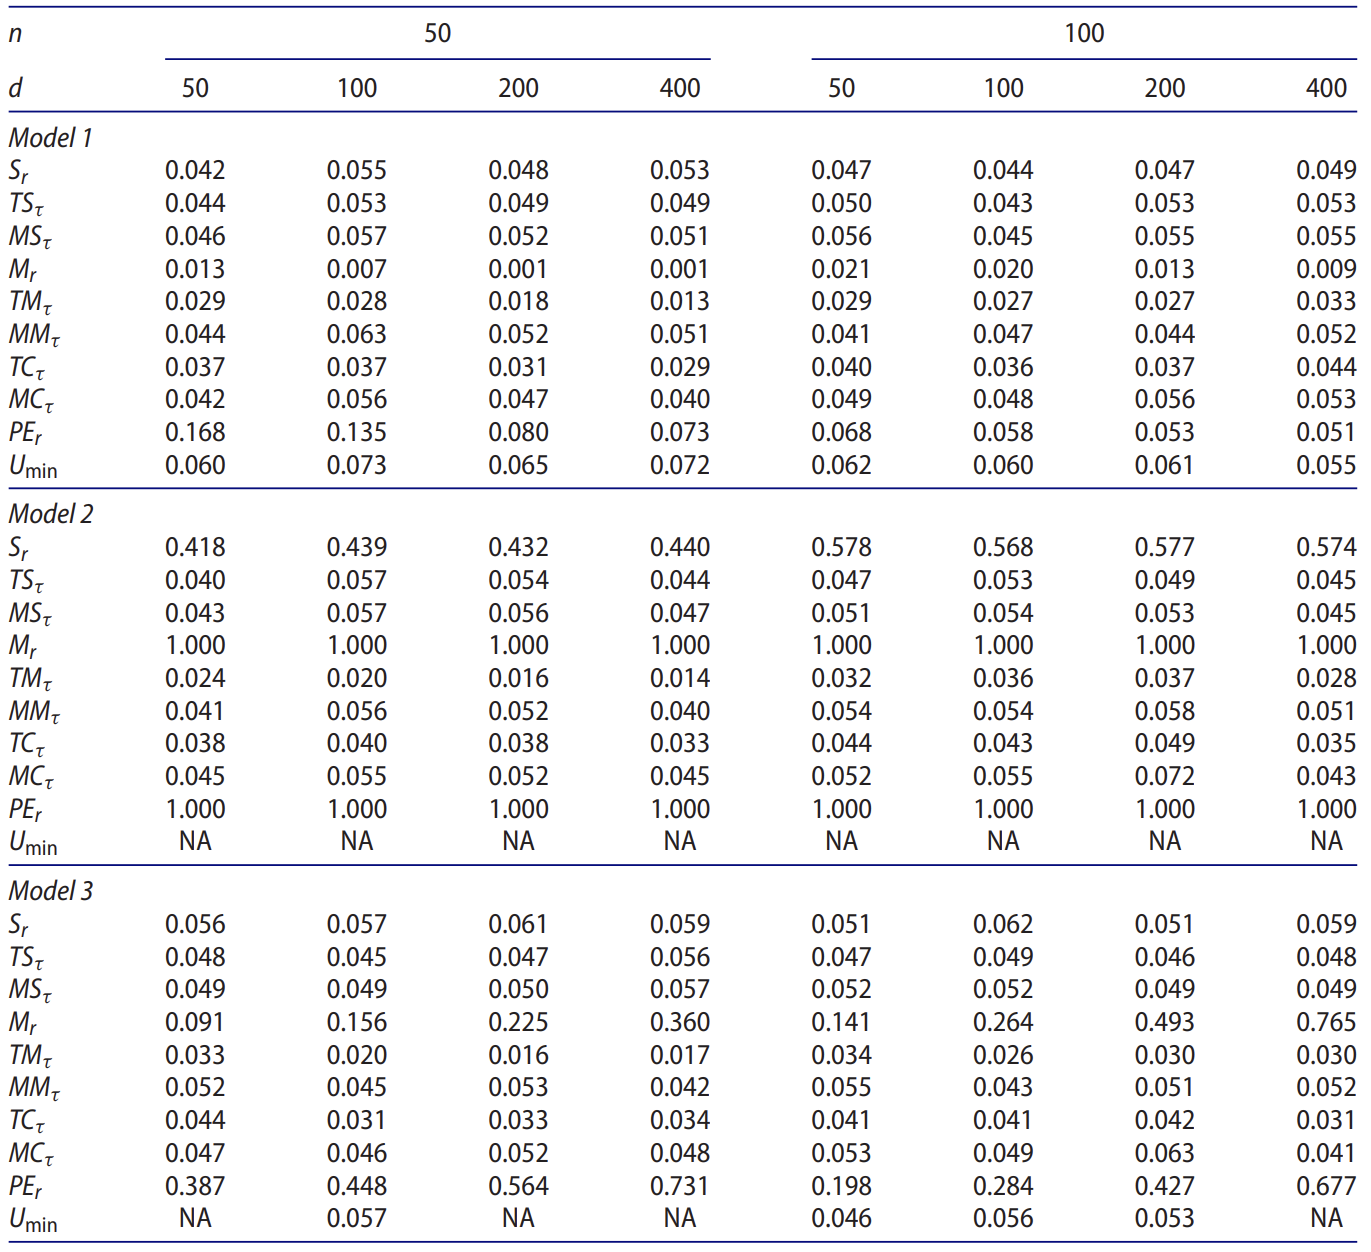
\includegraphics[width=0.8\linewidth,height=0.77\textheight]{Figures/Table1} 

}

\caption{Empirical sizes of tests}\label{fig:Table 1}
\end{figure}
\end{frame}

\begin{frame}{Results III}
\phantomsection\label{results-iii}
\begin{figure}

{\centering 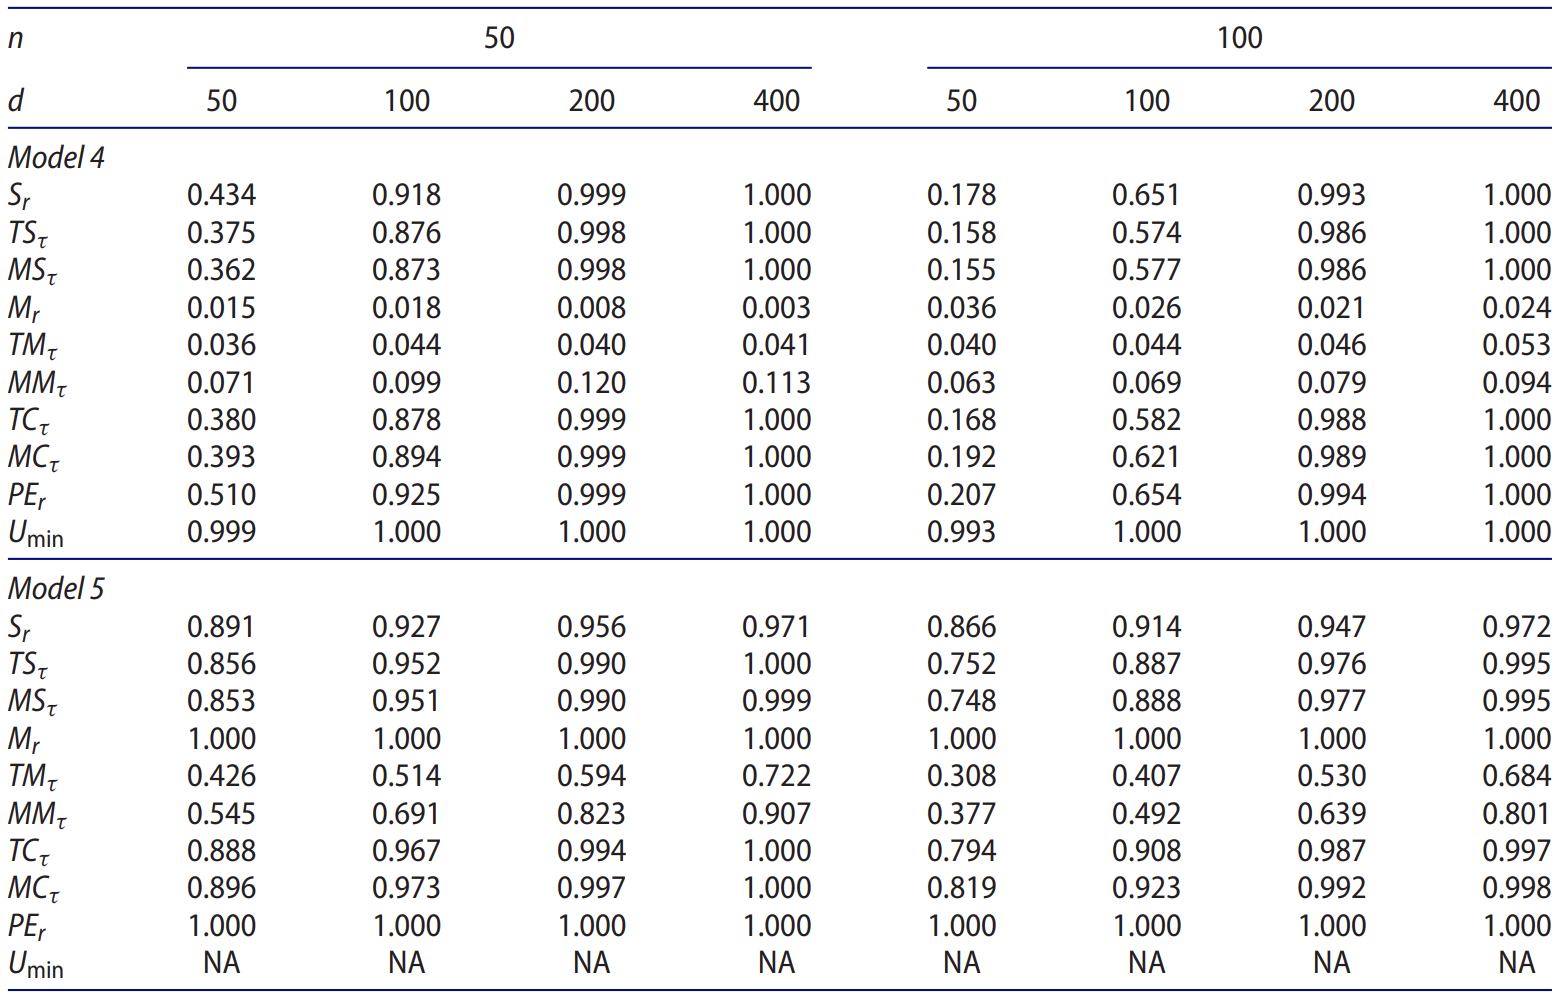
\includegraphics[width=0.8\linewidth]{Figures/Table2} 

}

\caption{Empirical powers of tests in dense cases.}\label{fig:Table 2}
\end{figure}
\end{frame}

\begin{frame}{Results IV}
\phantomsection\label{results-iv}
\begin{figure}

{\centering 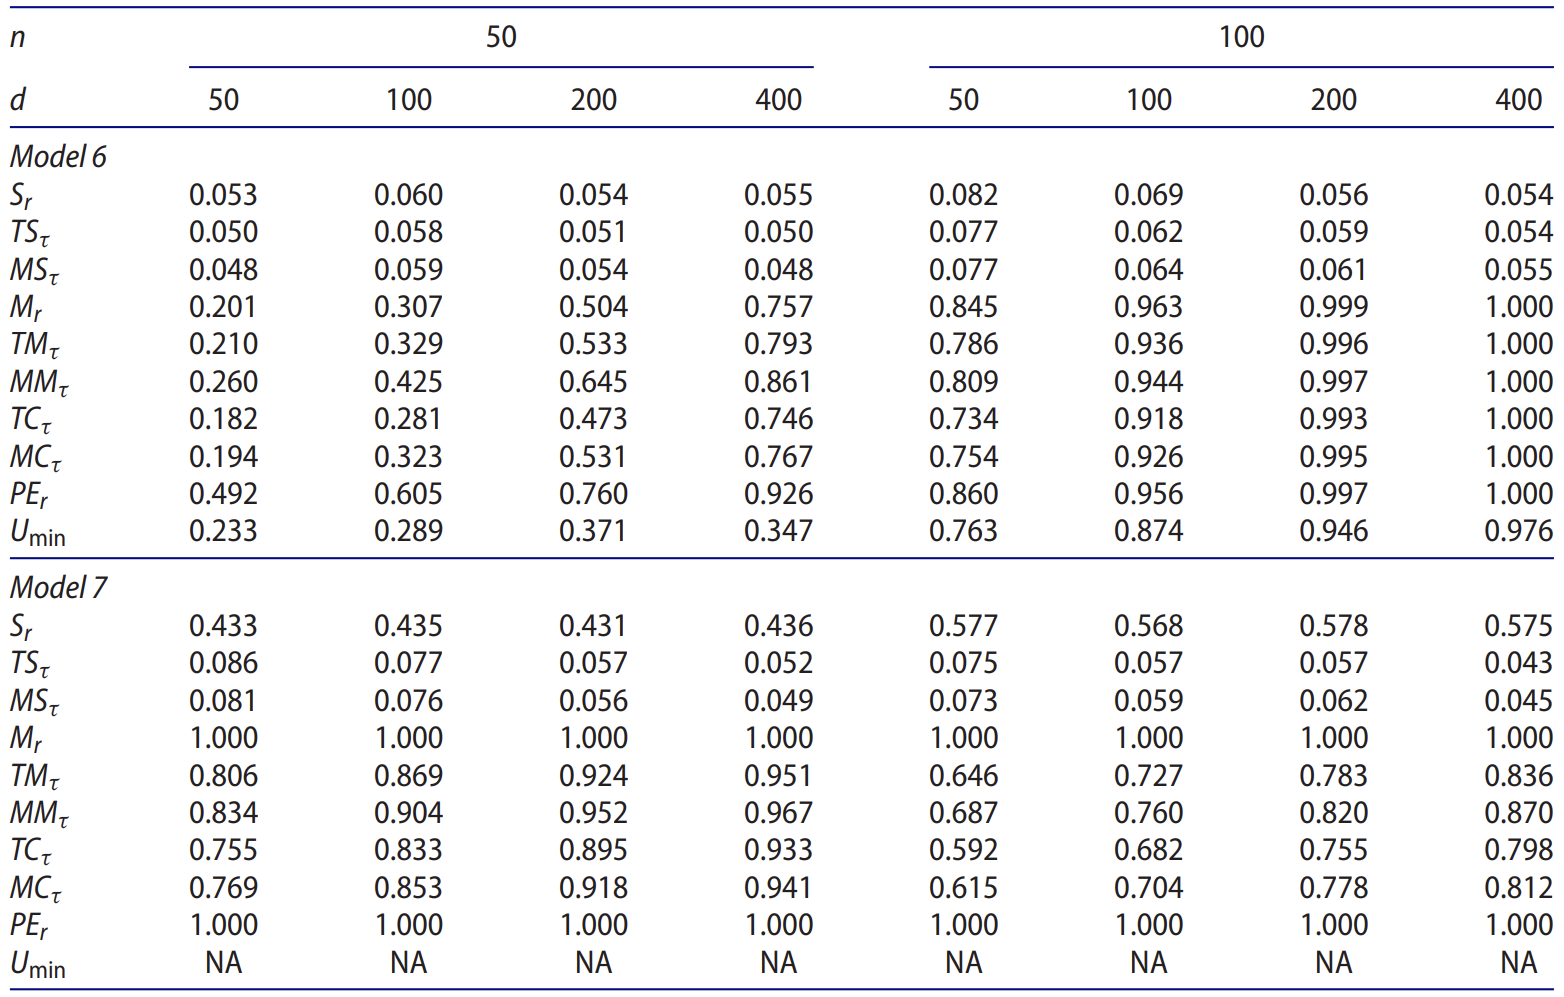
\includegraphics[width=0.8\linewidth]{Figures/Table3} 

}

\caption{Empirical powers of tests in sparse cases.}\label{fig:Table 3}
\end{figure}
\end{frame}

\begin{frame}{Results V}
\phantomsection\label{results-v}
\begin{figure}

{\centering 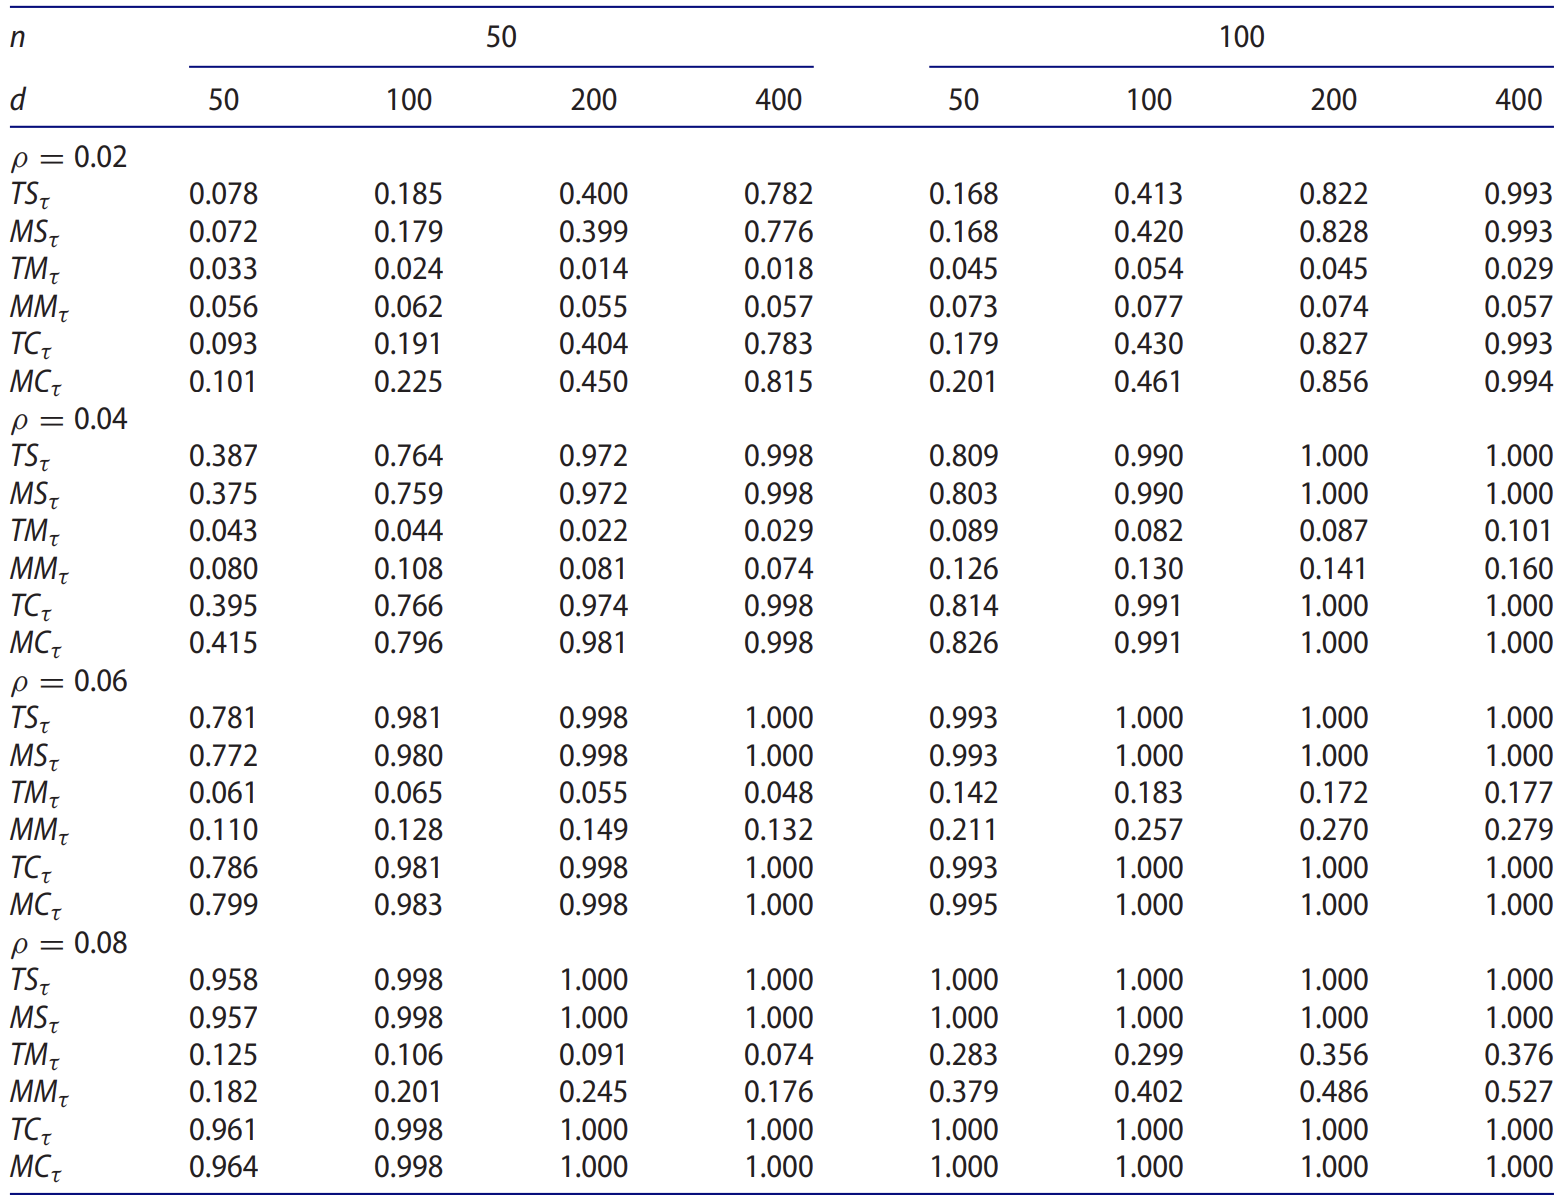
\includegraphics[width=0.8\linewidth,height=0.77\textheight]{Figures/Table4} 

}

\caption{Empirical powers under various strengths of dependence in dense cases.}\label{fig:Table 4}
\end{figure}
\end{frame}

\begin{frame}{Results VI}
\phantomsection\label{results-vi}
\begin{figure}

{\centering 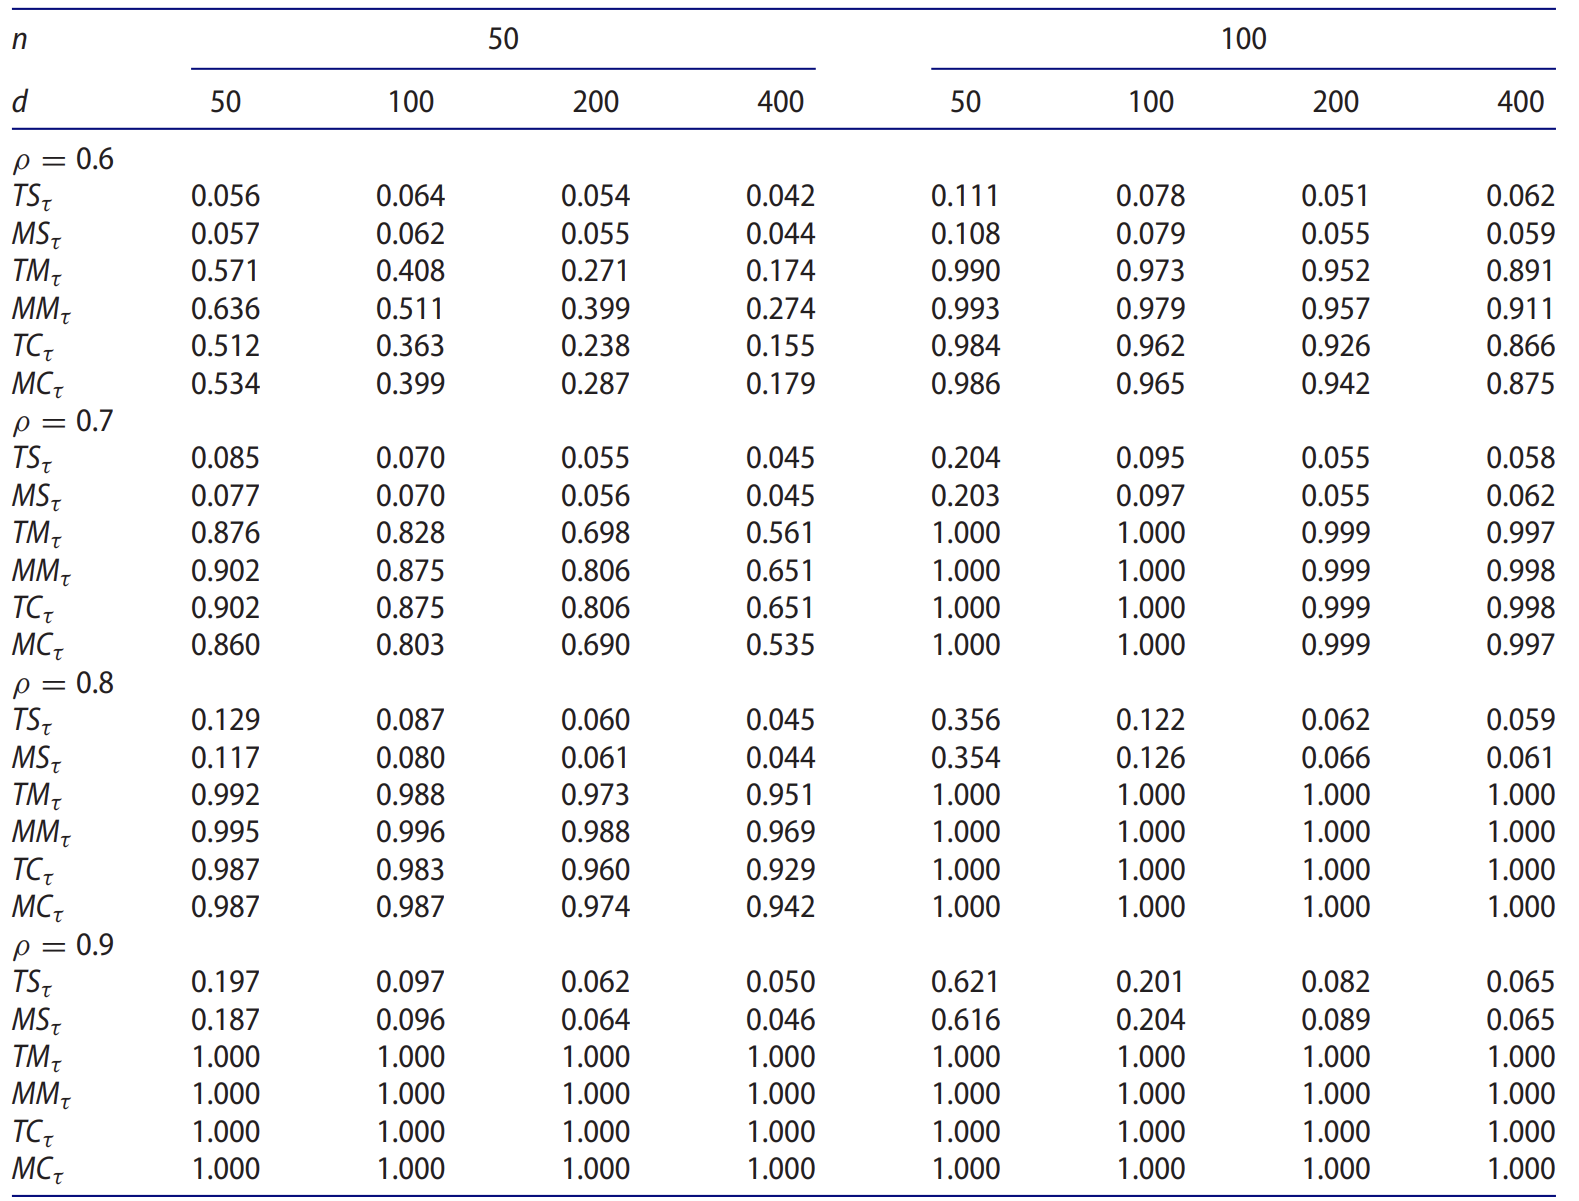
\includegraphics[width=0.8\linewidth]{Figures/Table5} 

}

\caption{Empirical powers under various strengths of dependence in sparse cases.}\label{fig:Table 5}
\end{figure}

\begin{block}{Empirics / Applications}
\phantomsection\label{empirics-applications}
\begin{itemize}
\tightlist
\item
  \textbf{Welding (4 vars, n=40):} rank-based rejects; Pearson fails.
\item
  \textbf{Biochemical (8 vars):} adaptive detects group differences.
\end{itemize}
\end{block}
\end{frame}

\begin{frame}{Conclusion}
\phantomsection\label{conclusion}
Rank-based adaptive tests are practical and robust; 2025 work
generalizes to sum-of-powers (Han, Ma, and Xie 2025).
\end{frame}

\begin{frame}{Next Steps}
\phantomsection\label{next-steps}
\begin{itemize}
\tightlist
\item
  Consulting applications (survey, environmental, biochemical).
\item
  Reflection: Kendall's \(\tau\) connects classic nonparametric tests to
  modern high-dimension inference.
\end{itemize}
\end{frame}

\begin{frame}[allowframebreaks]{References}
\phantomsection\label{references}
\scriptsize

\phantomsection\label{refs}
\begin{CSLReferences}{1}{0}
\bibitem[\citeproctext]{ref-ElShaarawi1992}
El-Shaarawi, A. H., and Stefan P. Niculescu. 1992. {``On Kendall's Tau
as a Test of Trend in Time Series Data.''} \emph{Environmetrics} 3 (4):
385--411.

\bibitem[\citeproctext]{ref-Fechner1897}
Fechner, Gustav Theodor. 1897. \emph{Kollektivmasslehre}. Leipzig:
Verlag von Wilhelm Engelmann.
\url{https://www.google.com/books/edition/Kollektivmasslehre/bgQZAAAAMAAJ?hl=en}.

\bibitem[\citeproctext]{ref-Hamed2011}
Hamed, K. H. 2011. {``The Distribution of Kendall's Tau for Testing the
Significance of Cross-Correlation in Persistent Data.''}
\emph{Hydrological Sciences Journal} 56 (5): 841--53.
\url{https://doi.org/10.1080/02626667.2011.586948}.

\bibitem[\citeproctext]{ref-Han2025}
Han, Lijuan, Yun Ma, and Junshan Xie. 2025. {``An Adaptive Test of the
Independence of High-Dimensional Data Based on Kendall Rank Correlation
Coefficient.''} \emph{Journal of Nonparametric Statistics} 37 (3):
632--56. \url{https://doi.org/10.1080/10485252.2024.2435852}.

\bibitem[\citeproctext]{ref-Kendall1938}
Kendall, M. G. 1938. {``A New Measure of Rank Correlation.''}
\emph{Biometrika} 30 (1/2): 81--93.
\url{https://www.jstor.org/stable/2332226}.

\bibitem[\citeproctext]{ref-Kruskal1958}
Kruskal, William H. 1958. {``Ordinal Measures of Association.''}
\emph{Journal of the American Statistical Association} 53 (284):
814--61. \url{https://doi.org/10.1080/01621459.1958.10501481}.

\bibitem[\citeproctext]{ref-Newson}
Newson, Roger. n.d. {``Parameters Behind {`Nonparametric'} Statistics:
Kendall's Tau, Somers' d and Median Differences.''} Working paper,
King's College London.

\bibitem[\citeproctext]{ref-Shi2024}
Shi, Xiangyu, Yuanyuan Jiang, Jiang Du, and Zhuqing Miao. 2024. {``An
Adaptive Test Based on Kendall's Tau for Independence in High
Dimensions.''} \emph{Journal of Nonparametric Statistics} 36 (4):
1064--87. \url{https://doi.org/10.1080/10485252.2023.2296521}.

\end{CSLReferences}
\end{frame}

\end{document}
